
\section{Проект расширения ассортимента продукции}

\textit{Краткая идея проекта.} Для повышения эффективности производства и реализации предприятия и повышения его доходов, необходимо расширить ассортимент производимой продукции за счет производства продуктов переработки молока и расширения рынков сбыта за счет новой продукции. Для этого необходимо открытие нового производства --- молочного цеха по переработке молока.



Продукция, которая будет производиться:
\begin{itemize}
	\item молоко пастеризованное; 
	\item напиток кисломолочный кефирный; 
	\item сметана или сливки питьевые; 
	\item творог; 
	\item сыр мягкий Адыгейский; 
	\item масло сливочное Крестьянское; 
	\item сыворотка.
\end{itemize} 

\textit{Цели и задачи проекта.} Целью данного проекта является запуск молочного цеха.

Задачи проекта:
\\
1. Покупка оборудования.
\\
2. Установка оборудования.
\\
3. Запуск нового цеха.
\\
4. Выпуск продукции.
\\

\textit{Этапы.}
Основные этапы проекта представлены на рисунке \ref{fig:1}
\begin{figure}[!h]
	\centering
	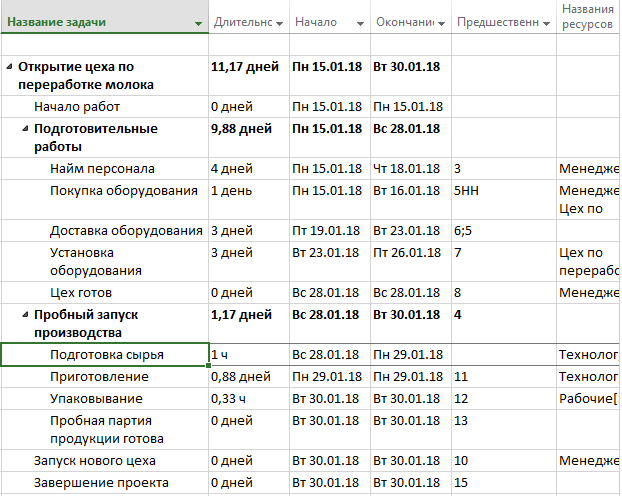
\includegraphics[width=1\linewidth]{fig1.png}
	\caption{Этапы проекта}
	
	\label{fig:1}
\end{figure}

\textit{Механизм реализации.}
Для реализации проекта в MicrosoftProject необходимо выполнить следующую последовательность действий.
\\
1. Начало проекта.
\\
2. Организация производства продуктов переработки молока.
\\
3. Приобретение цеха по переработке молока.
\\
4. Использование установки.
\\
5. Проект завершен.

\textit{Ресурсы}
\begin{figure}[!h]
	\centering
	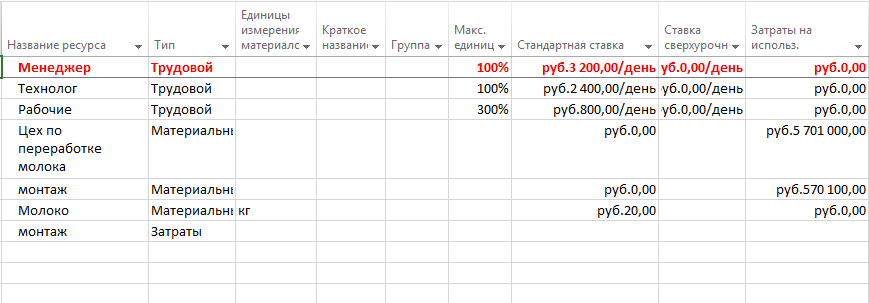
\includegraphics[width=1\linewidth]{fig13}
	\caption{Ресурсы проекта}
	\label{fig:fig12}
\end{figure}
Для реализации проекта необходимо собрать команду проекта:\\
Руководитель, технолог, рабочие.

\newpage
\textit{Диаграмма Ганта} показывает график работ по проекту.
\begin{figure}[!h]
	\centering
	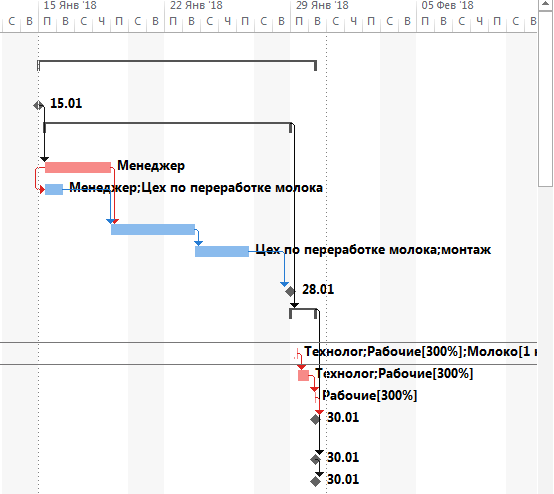
\includegraphics[width=1\linewidth]{fig12}
	\caption{Диаграмма Ганта}
	\label{fig:fig13}
\end{figure}
\newpage

\textit{Расчет экономической эффективности} и технико-экономические показатели приеведены в таблице \ref{my-label}

% Please add the following required packages to your document preamble:
% \usepackage{multirow}
\begin{table}[]
	\small
	\centering
	\caption{Технико-экономические показатели}
	\label{my-label}
	\setlength{\extrarowheight}{0.7mm}
	\begin{tabularx}{\textwidth}{|p{8.05cm}|p{8.05cm}|}
		\hline
		\multirow{6}{8cm}{Ассортимент и количество продукции, получаемой за сутки:} & молоко пастеризованное, фасованное в полиэтиленовые пакеты;     \\ \cline{2-2} 
																				& напиток кисломолочный кефирный, фасованный в полиэтиленовые пакеты; \\ \cline{2-2} 
																				& сметана или сливки питьевые, фасованные в пластиковые стаканчики;   \\ \cline{2-2} 
																				& творог, весовой;                                                    \\ \cline{2-2} 
																				& сыр мягкий Адыгейский, фасованный в пищевую пленку;                 \\ \cline{2-2} 
																				& масло сливочное Крестьянское, весовое.                              \\ \hline
		Объем перерабатываемого молока:                                         & 3 000 кг/сутки                                                      \\ \hline
		Количество обслуживающего персонала:                                    & 4 человека                                                          \\ \hline
		Энергопотребление цеха в сутки:                                         & 163 кВт/ч                                                           \\ \hline
		\multicolumn{2}{|l|}{Стоимость электроэнергии:}                                                                                               \\ \hline
		5 руб./кВт·ч х 163 кВт·ч х 0,5 = 407,5                                  & 408 руб./сутки                                                      \\ \hline
		Продолжительность месяца:                                               & 30 суток                                                            \\ \hline
		Зарплата одного работника:                                              & 800 руб./сутки                                                      \\ \hline
		Стоимость расходных материалов:                                         & 6000 руб./сутки                                                     \\ \hline
		Стоимость цеха с учётом НДС:                                            & 5 701 000 руб.                                                      \\ \hline
		Стоимость монтажных работ:                                              & 570 100 руб.                                                        \\ \hline
		Себестоимость молока:                                                   & 20 руб./кг.                                                         \\ \hline
		\multicolumn{2}{|l|}{Цена реализации готовых продуктов:}                                                                                      \\ \hline
		молоко;                                                                 & 34 руб./кг.                                                         \\ \hline
		напиток кефирный                                                        & 35 руб./кг.                                                         \\ \hline
		творог                                                                  & 150 руб./кг.                                                        \\ \hline
		сыр Адыгейский                                                          & 220 руб./кг.                                                        \\ \hline
		масло Крестьянское                                                      & 330 руб./кг.                                                        \\ \hline
		сметана                                                                 & 180 руб./кг.                                                        \\ \hline
		Расчет эффективности производства:                                      & Расчет дохода на 1 сутки:                                           \\ \hline
		Расчет затрат на 1 сутки:                                               & стоимость реализации готовой продукции                              \\ \hline
		стоимость молока: 3 000 кг. х 20 руб./кг =  60 000 руб.                 & молоко пастеризованное — 1294 кг х 34 руб/кг = 43 996 руб.          \\ \hline
		стоимость электроэнергии: 408 руб.                                      & напиток кисломолочный кефирный — 500 кг х 35 руб/кг = 17 500 руб.   \\ \hline
		зарплата работающих: 3 х 800 руб + 1200 руб = 3 600 руб.                & сметана или сливки питьевые — 136 кг х 180 руб/кг = 24 480 руб.     \\ \hline
		стоимость расходных материалов: 6 000 руб.                              & творог — 76 кг х 150 руб/кг = 11 400 руб.                           \\ \hline
																				& сыр мягкий Адыгейский — 50 кг х 220 руб/кг = 11 000 руб.            \\ \cline{2-2}
																				& масло сливочное Крестьянское — 19 кг х 330 руб/кг = 6 270 руб.      \\ \hline
		Всего:  70 008 руб.                                                     & Всего: 114 646 руб.                                                 \\ \hline
		\multicolumn{2}{|l|}{Расчет прибыли (за месяц): (114 646–70 008) х 30 = 1 339 140 руб.}                                                       \\ \hline
		\multicolumn{2}{|l|}{Расчет времени окупаемости:  (5 701 000 + 570 100) : 1 339 140 = 4,7 месяца}                                             \\ \hline
	\end{tabularx}
\end{table}































